% !TeX root = ../main.tex

\chapter{Fundamentos teóricos\label{chap:FUNDA}}

Este capítulo apresenta os conceitos necessários para a compreensão das técnicas e metodologias propostas neste trabalho, as quais são aplicadas em experimentos de recuperação de imagens pelo conteúdo. Destacamos ainda os métodos de extração de características do contorno das formas para obtenção de descritores. Enfatizamos neste capítulo as técnicas baseadas em assinaturas, em particular a curvatura, a distância ao centroide, a sequência de ângulos e os invariantes integrais. Utilizamos essas assinaturas para propor uma métrica de avaliação de similaridade entre formas. Apresentamos ainda as representações multiescala, a partir da qual desenvolvemos uma nova proposta de descritor multiescala de formas.


\section{\label{chap:CBIR} Sistemas de recuperação de imagens pelo conteúdo}

A disseminação dos sistemas de hardware embarcado com capacidade de coletar, armazenar e disponibilizar imagens digitais em redes de computadores, ampliou a demanda por aplicações de visão computacional em áreas como a medicina, indústria, segurança e biologia, entre outras. Dentre estas  demandas destacam-se as ferramentas efetivas de gerenciamento de informação multimídia que facilitam a organização e a busca automática desse tipo de conteúdo. 

Busca de imagens em grandes bases de dados multimídia é um dos serviços mais importantes disponibilizados pelos sistemas de gerenciamento de informação na atualidade. O método clássico para se prover tal serviço emprega a rotulação textual por palavras-chave. Nessa abordagem o usuário realiza buscas fornecendo informações textuais ao sistema. Esse último recupera a informação multimídia empregando métodos tradicionais de buscas textuais por palavras-chave. Atualmente, essa abordagem tem se tornado inviável devido ao grande volume de informação multimídia disponível na internet, o que torna o processo de anotação textual demasiadamente dispendioso. Ademais o processo de descrição textual é impreciso e sujeito a erros, uma vez que diferentes indivíduos tendem a interpretar e descrever uma mesma imagem subjetivamente e, portanto, empregando diferentes palavras-chave na descrição. Os sistemas de recuperação de imagens pelo conteúdo (\emph{CBIR}) foram propostos em resposta a essas dificuldades. Nesses sistemas o processo de busca utiliza o conteúdo visual das imagens ao invés da rotulação textual. 

\subsection{Arquitetura dos sistemas \emph{CBIR}}

Sistemas \emph{CBIR} empregam o conteúdo visual das imagens para formar uma base de dados de representações na forma de vetores de características. A busca é então realizada com o usuário fornecendo ao sistema uma imagem, ou figura de consulta, a qual também é representada vetorialmente. Assim, através da avaliação da similaridade existente entre as representações da imagem de consulta e das imagens da base, o sistema procura retornar ao usuário as imagens que sejam do seu interesse. Dependendo das particularidades da aplicação, esse padrão de consulta, que corresponde também a uma imagem, pode ser um esboço, um modelo ou uma cópia exata do que se deseja procurar \cite{Smeulders:2000}.

\begin{comment}
Sistemas \emph{CBIR} realizam buscas em bases multimídia utilizando o conteúdo visual das imagens, visando recuperar imagens que sejam do interesse do usuário mediante um padrão de consulta especificado. O campo das pesquisas em recuperação de imagens pelo conteúdo é vasto e relativamente recente.
\end{comment}


A Figura \ref{fig:cbir} apresenta a arquitetura de um sistema \emph{CBIR} clássico, sendo este composto pelos seguintes componentes \cite{Torres:2006}:

\begin{alineas}
\item Módulo de interação com usuário: através desse módulo o usuário fornece como entrada ao sistema uma imagem de consulta e visualiza, como saída, os resultados das buscas. É também através desse módulo que são realizadas a inserção e a remoção de imagens da base de imagens, sendo esse último processo, destacado em linhas tracejadas, realizado pelo administrador do sistema;  
\item Módulo de processamento de busca: esse módulo engloba grande parte da funcionalidade do sistema \textit{CBIR}, sendo esse composto pelos seguintes submódulos:
\begin{alineas}
\item Extração de características: contempla os algoritmos computacionais responsáveis em obter uma representação matemática, na forma de vetor de características, dos atributos visuais das imagens como cor, textura e forma;
\item Avaliação de similaridade: contempla o método empregado para a avaliação do grau de similaridade existente entre as imagens a partir de suas respectivas representações vetoriais;
\item Ordenação dos resultados: método para seleção das imagens que serão apresentadas ao usuário conforme o grau de similaridade ao padrão fornecido;
\end{alineas} 
\item Base de imagens: repositórios aonde estão contidas as imagens, bem como suas correspondentes representações vetoriais.
\end{alineas}

\begin{figure} 
\centering
\caption{\label{fig:cbir} Arquitetura de um sistema \emph{CBIR}.}
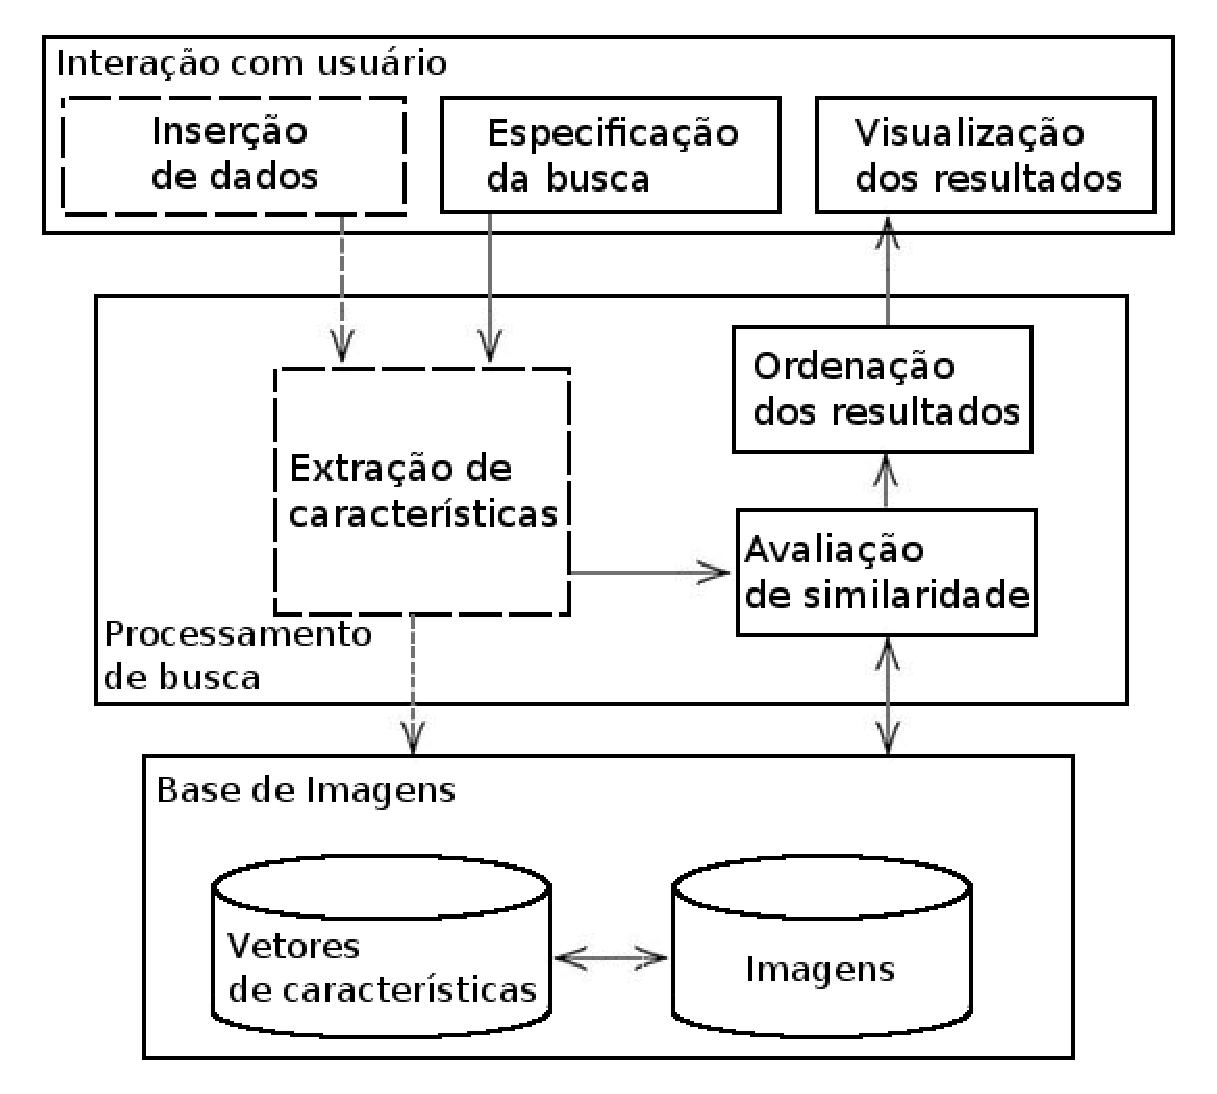
\includegraphics[width=0.65\textwidth]{cbir.eps}
\legend{Fonte: \citeonline{Torres:2006}.}
\end{figure}
 
Neste trabalho enfatizamos os processos de extração de características e de avaliação de similaridade em \emph{CBIR}, sendo esses processos destacados nas subseções a seguir.

\subsection{Extração de características}

O processo de extração de características das imagens forma é fundamental para os sistemas \emph{CBIR}. Tal processo se dá através de operações de processamento de imagens, cujo objetivo é extrair informação que seja semanticamente relevante dos atributos da imagem para a realização das buscas por similaridade de conteúdo. Os atributos comumente empregados para extração de características em \emph{CBIR} são a cor, a textura, a forma e a localização espacial dos elementos constituintes de uma imagem. 

A cor é o atributo mais empregado em \emph{CBIR}, pois a mesma permite discriminar uma ampla gama de imagens. Quando se utiliza esse atributo deve se considerar que o registro da cor em uma imagem varia consideravelmente com a orientação da superfície imageada, o posicionamento da câmera, a posição da fonte de iluminação e a maneira como a luz interage com os objetos imageados \cite{Smeulders:2000}. Ademais, a percepção humana da cor é um assunto complexo que ainda não está completamente elucidado \cite{Smeulders:2000}. De acordo com \citeonline{Torres:2006}, as técnicas de descrição por cores podem ser agrupadas em duas grandes classes dependendo se a informação de cor é codificada correlacionada com a sua distribuição espacial ou não. 

\begin{comment}Esses mesmos autores exemplificam como técnicas que não levam em consideração a distribuição espacial das cores os histogramas e os momentos de cores. 
\end{comment}

Atributos de textura são úteis na recuperação de imagens de satélites, bem como na busca de documentos digitalizados \cite{Smeulders:2000}. A textura é definida em termos de estruturas formadas por grupos de pixels que aparecem na imagem com certa periodicidade ou aleatoriedade. O método já consagrado para descrição de características de texturas é a matriz de coocorrência proposta por \citeonline{4309314}. No entanto, métodos baseados em transformações wavelet têm sido utilizados \cite{5376587}, mais notoriamente a transformada wavelet de Gabor \cite{531803}. Outra técnica que tem sido explorada na atualidade para descrição de texturas é a dimensão fractal multiescala \cite{Florindo:2013}. 

Informação relativa à localização espacial dos elementos de uma imagem permite, por exemplo, recuperar imagens de cenas fotográficas de paisagens externas, aonde distingue-se a localização do céu na região superior da imagem. Ademais, imagens fotográficas também tendem a apresentar em seu centro alguma informação significativa que difere do entorno da imagem, sendo essa informação útil no processo de recuperação de imagens de fotografias de pessoas, animais, etc.

A forma é uma característica intrínseca das imagens que é amplamente explorada pelo sistema de visão dos primatas para o reconhecimento de objetos. Progressos significativos têm sido alcançados no desenvolvimentos de sistemas de recuperação de imagens pelo conteúdo baseados nesse atributo.

Dentre as abordagens empregadas na obtenção de representações a partir das formas, a mais popular é a que as representa através de vetores de características. Tal representação permite que a similaridade entre as formas seja avaliada através de medidas de distância entre vetores. No entanto, a representação por vetores de características é pouco discriminativa, o que limita a sua acurácia em aplicações \emph{CBIR}.

Na representação estrutural, as formas são divididas em um conjunto de partes constituintes, sendo cada parte representada individualmente através de vetores de características. O descritor é composto a partir desses vetores e da relação existente entre as partes, representadas através de estruturas de dados como grafos, árvores ou cadeias de caracteres. Uma vez que esses métodos comparam as formas a partir das suas estruturas, esses conseguem uma boa acurácia, porém a um custo computacional elevado.

% {\color{red}Métodos de representação de formas por transformação empregam transformadas como wavelet, Fourier e Espaço-Escala para descrever as formasESTA PEDINDO PARA CITAR TRABALHOS AQUI, OU ENTAO ELIMINA. Em \emph{CBIR}, o custo computacional das buscas deve levar em consideração o custo de se aplicar a transformada à forma de consulta. }


O descritor do contorno da forma SC ou \emph{shape context} \cite{Belongie:2002} avalia a similaridade entre formas por correspondência de pontos. Esse descritor caracteriza a distribuição dos demais pontos do contorno em relação a um ponto de referência para cada ponto do contorno tomado como referência. 
Os métodos que usam correspondência, ou alinhamento, representam as formas diretamente no domínio espacial. Esses métodos determinam o grau de similaridade entre duas formas tentando alinhá-las de modo a medir a diferença residual existente entre as mesmas.


\begin{comment}
As abordagens empregadas na obtenção de representações a partir das formas podem ser classificadas em 3 grandes categorias:

\begin{alineas}

\item representação por vetor de características: É a técnica mais popular de representação. Neste método, a forma é representada através de um vetor numérico e a similaridade entre as formas é avaliada através de uma distância entre vetores. 

\item representação por transformação: deformações são realizadas em uma forma a fim de transformá-la em outra. A similaridade entre as formas é medida pelo esforço necessário para se realizar a transformação.  

\item representação relacional: Nesta abordagem as formas são divididas em um conjunto de partes constituintes. Cada parte é individualmente representada através de vetores de características. O descritor é composto a partir destes vetores e da relação existente entre as partes.
\end{alineas}

Técnicas de representação por vetores de características são classificadas em duas grandes classes: técnicas baseadas em região e técnicas baseadas em contorno.
\end{comment}

\subsection{Medidas de similaridade}
O processo de recuperação de imagens pelo conteúdo requer que alguma medida seja empregada na avaliação da similaridade entre as representações das imagens. Nas técnicas de extração de características que resultam em representações vetoriais, as medidas de distância entre vetores são comumente empregadas para este fim. Desta forma, o grau de similaridade entre duas representações guarda uma relação inversa com a medida de distância correspondente. 

 Uma medida entre dois vetores $p$ e $q$ é considerada uma distância quando satisfaz as seguintes propriedades \cite{Ullah1996}: 

\begin{alineas}
\item Positividade: $d(p,q) \geq 0$;  
\item Unicidade: $d(p,q) = 0 \Rightarrow p = q$;
\item Simetria: $d(p,q) = d(q,p)$;
\item Desigualdade triangular: $d(p,r) + d(r,q) \geq d(p,q)$.
\end{alineas}

Para as representações vetoriais dentro de um mesmo espaço dimensional, distâncias entre vetores, como as apresentadas na Tabela \ref{tbl:distance}, são empregadas. Casos aonde a representação das imagens resulta em descrições de dimensões distintas, técnicas mais elaboradas, que utilizam programação dinâmica, são necessárias. Dentre essas técnicas a \emph{DSW} (\emph{Dynamic space warping})\cite{Alajlan20117,{4815272}} tem sido empregada na avaliação de similaridade entre formas, a partir de assinaturas extraídas dos seus contornos. 

\begin{table}
\centering
\caption{\label{tbl:distance}Medidas de distância entre vetores}
\begin{tabular}[]{ll}
\hline
Medida de distância&Fórmula matemática\\
\hline
Distância de Minkowski&$d(x,y) = \Big[\sum\limits_{i=1}^{n}(x_i-y_i)^m\Big]^\frac{1}{m}$\\
Distância euclidiana&$d(x,y) = \Big[\sum\limits_{i=1}^{n}(x_i-y_i)^2\Big]^\frac{1}{2}$\\
Distância city-block&$d(x,y)= \sum\limits_{i=1}^{n}|x_i-y_i|$\\
Distância Chebyshev&$d(x,y)= \max\limits_{i}|x_i-y_i|$\\
Separação angular&$d(x,y)=\frac{\sum\limits_{i=1}^n{x_iy_i}}{\Big[\sum\limits_{i=1}^n{x_i^2}\sum\limits_{i=1}^n{y_i^2}\Big]^\frac{1}{2}}$\\
Canberra&$d(x,y) = \sum\limits_{i=1}^n\frac{|x_i-y_i|}{x_i+y_i}$\\
\hline
\end{tabular}
\end{table}

\section{\label{chap:contour}Descritores do contorno das formas}

Os estímulos visuais, ao qual os sistemas de visão biológicos estão submetidos, apresentam um elevado grau de redundância de informação. No processamento dessa informação, tais sistemas buscam eliminar essas redundâncias, retendo apenas a quantidade de informação necessária para o desempenho da tarefa requerida.  

Em visão computacional e reconhecimento de padrões, dá-se o nome a esse processo de eliminação das redundâncias de extração de características. Esta etapa de baixo nível busca encontrar informação relevante em uma imagem e representá-la convenientemente para a realização de uma tarefa específica de visão computacional. Uma vez que o processo de extração de características determina o desempenho de um sistema de visão computacional, este recebe especial atenção no desenvolvimento de tais sistemas.

Dentre os atributos dos quais se realizam a extração de características, a forma é considerada a mais relevante em diversas aplicações de visão artificial pela riqueza de informações que esta possui. Uma forma é obtida quando um objeto de interesse é identificado e segmentado em uma imagem. 
 De acordo com \citeonline{Zhang:2004}, para que se obtenha uma representação conveniente com base nesse atributo, deve-se buscar por informações que tenham importância em sua percepção, seja no contorno ou na região que a delimita. 

Obter uma representação, ou descrição, de objetos a partir de formas planas é uma tarefa complexa. Isso porque quando projetamos os objetos tridimensionais do mundo real em duas dimensões, perdemos as informações de uma das dimensões. Como resultado temos uma representação bidimensional parcial do objeto projetado. O problema torna-se ainda mais complexo se levarmos em conta que a forma é frequentemente corrompida por ruídos, defeitos, distorções arbitrárias e oclusões.

\citeonline{Zhang:2004} classificam as técnicas de representação de formas em duas grandes classes de métodos: os baseados em contorno e os baseados em região. Nos métodos baseados em região as características são extraídas de toda região da forma, enquanto que nos métodos baseados em contorno, as características são extraídas apenas da borda. Os referidos autores ainda subdividem cada classe de métodos em métodos estruturais e globais. Essa subdivisão é baseada em se a forma como um todo é utilizada na representação ou se a representação é obtida de partes, segmentos e seções das formas. 

A Figura \ref{fig:folha_contorno1} ilustra as etapas envolvidas no processo de representação de uma forma. Temos nesse caso a segmentação da imagem por limiar seguida da extração do contorno. Com base no contorno, obtém-se uma variedade de representações, na forma de sinais, adequadas para as tarefas de comparação, classificação e reconhecimento de formas.

Neste trabalho  enfatizamos a aplicação de técnicas de processamento de sinais para a obtenção de representações globais do contorno das formas, uma vez que tais técnicas têm sido empregadas com sucesso para esse propósito \cite{Costa:2009}. 

\begin{comment}
Técnicas baseadas em contorno de formas exploram apenas a região da borda da forma. Há dois tipos de abordagens para extração de características do contorno das formas: global e estrutural. Na abordagem global a forma não é dividida em subpartes e um vetor de características que representa toda a borda é obtido para representar a forma. Na abordagem estrutural a borda da forma é particionada em segmentos, denominados de primitivas mediante algum critério. A representação final é geralmente uma cadeia de caracteres, um grafo ou uma árvore.
\end{comment}



%representar uma forma consiste em caracterizá-la através de um conjunto de características que permitam reconstrui-la exatamente ou com um certo grau de precisão. Os mesmos autores classificam os métodos de representação das formas em três grandes grupos: por contorno, por região e por transformação.
    

\begin{figure} 
\caption{\label{fig:folha_contorno1} Obtenção da forma e do contorno da imagem de uma folha.}
%\includegraphics[width=\textwidth,clip,trim=12mm 188mm 27mm 75mm]{figura_folha.png}
\includegraphics[width=\textwidth,clip,trim=10mm 145mm 36mm 26mm]{figura_folha_v3.png}
%\legend{Fonte: próprio autor}
\end{figure}

\subsection{\label{sec:Assinatura}Representação paramétrica do contorno e curvatura
}

\citeonline{Costa:2009} definem assinatura de uma forma como sendo um sinal discreto unidimensional que descreve algumas das características do seu contorno ou da sua região. Devido a redução de dimensionalidade, as assinaturas do contorno são representações compactas das formas. Estas assinaturas podem ser utilizadas diretamente como descritores, porém o custo computacional envolvido em sua comparação direta é elevado. Isso porque as assinaturas, em geral, não são totalmente insensíveis a rotação, translação e escalamento das formas, bem como variam no total de amostras conforme varia a resolução das imagens. Algumas assinaturas são mais sensíveis a ruído e a pequenas distorções dos contornos, tornando necessário realizar filtragens. Embora melhore a robustez, tal processo acarreta em alguma perda de informação.

% Várias assinaturas vêm sendo empregadas na literatura para descrição de formas nas mais diversas aplicações, tais como a distância ao centroide, as coordenadas complexas, ângulo tangente, ângulo acumulativo, curvatura, área e comprimento da corda \cite{Zhang:2004}.

% \subsubsection*{\label{sec:Rep_par}Coordenadas paramétricas}
A representação por coordenadas paramétricas consiste na otenção das coordenadas dos pontos amostrados do contorno, representados a partir de um sistema de coordenadas preestabelecido, percorrendo-o sequencialmente em sentido horário ou anti-horário. Para o contorno discreto $\mathbf{C}$, com $N$ amostras, representado num sistema de coordenadas cartesianas, tal processo origina um conjunto de tuplas $\mathbf{C}[n] = \big(\mathbf{x}[n]\:\text{,}\:\mathbf{y}[n]\big)$, $n \in {\{0\:\text{,}\:1\:\text{,}\:\dotsc\:\text{,}\:N-1\}}$, cujas componentes $\mathbf{x}[n]$ e $\mathbf{y}[n]$ são sinais discretos vetoriais das coordenadas amostradas do contorno.

Na Figura \ref{fig:folha_contorno} estão representados os sinais obtidos para o contorno da folha da Figura \ref{fig:folha_contorno1} com a amostragem $N = 280$ pontos. Em vermelho está destacado o ponto de origem aonde a varredura, em sentido horário, se inicia. Os dois pontos observados aonde a evolução do sinal $\mathbf{x}[n]$ inverte sua tendência (de crescente para decrescente e de decrescente para crescente) correspondem aos pontos mais salientes da folha. Já o platô observado no sinal $\mathbf{y}[n]$ corresponde a região da parte inferior da folha, em que quase não se observa variações do contorno ao longo do eixo $Y$.
   
\begin{figure} 
\caption{\label{fig:folha_contorno} Processo de obtenção da representação paramétrica do contorno da folha da Figura \ref{fig:folha_contorno1}.}
\includegraphics[width=\textwidth,clip,trim= 12mm 30mm 10mm 77mm]{figura_folha_v3.png}
%\legend{Fonte: próprio autor}
\end{figure}

Outra representação paramétrica para o contorno é obtida compondo-se um sinal complexo $\mathbf{z}[n] = \mathbf{x}[n] + j\mathbf{y}[n]$, $j = \sqrt{-1}$, $n \in {\{0\:\text{,}\:1\:\text{,}\:\dotsc\:\text{,}\:N-1\}}$. Essa representação é conveniente quando se deseja realizar extração de características do contorno através de operações de processamento de sinais. A Figura \ref{fig:folha_complex} ilustra o módulo e a fase da representação complexa do contorno da folha da Figura \ref{fig:folha_contorno1}. 

\begin{figure} 
\caption{\label{fig:folha_complex} Representação paramétrica do contorno da forma da folha na imagem da Figura \ref{fig:folha_contorno1} como sinal complexo.}
\centering
\includegraphics[width=0.75\textwidth]{folha_complex_v3.png}
%\legend{Fonte: próprio autor}
\end{figure} 

Embora sejam descritivas, as representações por coordenadas paramétricas apresentam o inconveniente de não serem invariantes a translação, rotação ou escalamento das formas, porém, outras assinaturas com tais propriedades podem ser derivadas a partir dessas mesmas \cite{Kindratenko:2003}.

% \subsubsection*{Curvatura\label{sec:curvatura}}

A curvatura é uma assinatura do contorno da forma com importantes propriedades geométricas, o que motiva sua utilização para obtenção de descritores. Há evidências biológicas de que as propriedades desta assinatura sejam exploradas pelo sistema de visão dos primatas nas tarefas de reconhecimento de formas \cite{Costa:2009}. Na Tabela \ref{tbl:curv} estão destacadas as principais propriedades que a curvatura apresenta.  

\begin{table}
\centering
\caption{\label{tbl:curv} Propriedades da curvatura e as características geométricas que essas representam.}
\begin{tabular}[]{ll}
\toprule
\multicolumn{1}{c|}{Propriedade} & \multicolumn{1}{c}{Característica da forma}\\ 
\hline
Máximo valor absoluto & Ponto saliente \\
Máximo valor positivo & Saliência convexa \\
Mínimo valor negativo & Saliência côncava \\
Valores constantes e nulos & Segmentos retilíneos \\
Valores constantes e não nulos & Segmentos circulares \\
Cruzamentos de zero & Pontos de inflexão \\ \bottomrule
\end{tabular}
\legend{Fonte: \citeonline{Costa:2009}}
\end{table}

A função curvatura ($K(l)$), para uma curva contínua fechada $C = \big(x(l)\:\text{,}\:y(l)\big)$,  cujo perímetro é $L$ e que encontra-se parametrizada em $l \in [0\text{,}L]$, é definida como sendo \cite{Kindratenko:2003}:

\begin{equation} \label{eq:curvatura}
K(l) = \frac{x^{'}(l)y^{''}(l)-x^{''}(l)y^{'}(l)}{((x^{''}(l))^{2}+(y^{''}(l))^{2})^{\frac{3}{2}}}\text{,}
\end{equation}

\noindent 
sendo $\big(x^{'}(l) \text{, }y^{'}(l)\big)$ e $\big(x^{''}(l)\text{ , }y^{''}(l)\big)$ as derivadas primeira e segunda das coordenadas paramétricas da curva, respectivamente.

Sob o aspecto computacional, o cálculo da curvatura do contorno de uma forma requer que o mesmo seja espacialmente amostrado e discretizado. Tal processo torna o cálculo das derivadas da Equação \ref{eq:curvatura} sensível ao ruído e inviável, o que limita a aplicação direta da curvatura para a obtenção de descritores. 

A Figura \ref{fig:cir1} ilustra tal efeito para uma imagem de forma circular. A Figura \ref{fig:cir1}a representa o gráfico da curvatura teórica, obtida analiticamente, pela aplicação da Equação \ref{eq:curvatura} ao contorno parametrizado do círculo de mesmo raio ao do círculo da Figura \ref{fig:cir1}b. Já na  Figura \ref{fig:cir1}c, temos a curvatura obtida computacionalmente a partir do contorno discreto extraído do círculo da Figura \ref{fig:cir1}b. Nota-se que a curvatura da Figura \ref{fig:cir1}a (analítica) tem um valor constante $K(l) = \frac{1}{r}$, sendo $r$ o raio do círculo central, enquanto que a curvatura Figura \ref{fig:cir1}c (computacional) varia significativamente em torno do valor analítico esperado, como mostra a Figura \ref{fig:cir1}. 

\begin{figure}[h!]
  \caption{\label{fig:cir1} Efeito do ruído na estimativa computacional da curvatura para uma forma circular.}
  \centering
  \includegraphics[width=\textwidth, clip, trim=20mm 5mm 0mm 0mm]{curv_cir.png}
  %\legend{Fonte: próprio autor}
\end{figure}

Diversas estratégias foram propostas na literatura para contornar o problema da sensibilidade ao ruído do cálculo computacional da curvatura. Trabalhos clássicos, como os de \citeonline{5009188} e \citeonline{LynnBeus1987291} estimam a curvatura a partir do ângulo formado entre vetores obtidos a partir dos pontos do contorno. \citeonline{Cazals:2003} e \citeonline{Shi20022051} apresentaram trabalhos que utilizavam métodos para estimação da curvatura por interpolação de pontos. 

\citeonline{149591} introduziram um método que suaviza o contorno, através da convolução do mesmo com um filtro gaussiano, antes de se calcular a curvatura.

\begin{figure}[h!]
 \caption{\label{fig:curv_folha} Curvatura estimada do contorno da folha da Figura \ref{fig:folha_contorno1} através de método computacional.}
  \centering
  \includegraphics[width=0.75\textwidth]{curv_folha_v2.png}
%\legend{Fonte: próprio autor}
\end{figure}

A Figura \ref{fig:curv_folha} mostra a curvatura estimada, para o contorno da folha da Figura \ref{fig:folha_contorno1}, através do método proposto por \citeonline{149591}. O contorno foi previamente suavizado com um filtro gaussiano com desvio padrão $\sigma = 20$. Os pontos aonde a curvatura apresenta os picos em destaque correspondem aos pontos salientes da folha. 

\begin{comment}
Particularmente, métodos de extração de características multiescala do contorno a partir da curvatura conseguem superar o problema supracitado aplicando filtragens passa-baixa a representação paramétrica do contorno antes de se calcular a curvatura. 
\end{comment}

% {\color{magenta}
% \subsubsection*{Distância ao centroide}
% Uma assinatura simples pode ser obtida calculando-se a distância de cada coordenada do contorno ao centroide da forma. Esse último consiste, para um contorno discreto de $N$ amostras, em um vetor calculado, a partir das coordenadas do contorno, pela seguinte equação: 

% \begin{equation}
% \big(x_{c}\:\text{,}\:y_{c}\big) = \Big(\frac{1}{N}\sum^{N}_{i=0}{\mathbf{x}[i]}\:\text{,}\:\frac{1}{N}\sum^{N}_{i=0}{\mathbf{y}[i]}\Big)\text{.}
% \end{equation}

% O sinal da distância ao centroide $\mathbf{dc}[n]$ é dado por:

% \begin{equation}
% \mathbf{dc}[n] = \sqrt{(\mathbf{x}[n] - x_c)^2 + (\mathbf{y}[n] - y_c)^2}\text{.}
% \end{equation}

% Essa assinatura tem a propriedade de ser invariante a translação da forma, o que a torna independente do sistema de coordenadas adotado na parametrização do contorno. Embora não seja invariante a escala e a rotação, tais invariâncias podem ser obtidas, como sugerem alguns trabalhos. 

% Empregando um processo de subamostragem e de normalização pelo maior valor, \citeonline{Wang:2000} tornam essa assinatura invariante a escala. Para se alcançar invariância a rotação os referidos autores sugerem que, no processo de avaliação de similaridade entre duas assinaturas, seja realizado o deslocamento cíclico de uma das assinaturas até que se obtenha a maior similaridade.

% Já \citeonline{Zhang:02} utilizam a distância ao centroide como assinatura para se obter os descritores de Fourier. Tal estratégia garante as propriedades de invariância a rotação e a escala.

% \begin{figure}[h!]
%   \caption{\label{fig:cd} Assinatura da distância ao centroide para o contorno da folha da Figura \ref{fig:folha_contorno1}}
%   \centering
%   \includegraphics[width=0.75\textwidth]{cd_v2.png}
%   %\legend{Fonte: próprio autor}
% \end{figure}

% A Figura \ref{fig:cd} ilustra a assinatura da distância ao centroide para a folha da Figura \ref{fig:folha_contorno1}. Neste exemplo, a assinatura foi normalizada a partir da distância máxima ao centroide, que corresponde ao ponto vermelho demarcado tanto no gráfico como no contorno. 

% \subsubsection*{Sequência de ângulos}

% A assinatura de sequência de ângulos é obtida a partir do ângulo formado entre vetores construídos a partir das coordenadas do contorno parametrizado conforme ilustrado na Figura \ref{fig:angulo}. 

% Para um dado ponto pertencente ao contorno, de coordenadas $(x_i\:\text{,}\:y_i)$, obtemos os vetores $\overrightarrow{v_1}$ e $\overrightarrow{v_2}$. O primeiro vetor é formado pela diferença entre as coordenadas $(x_i\:\text{,}\:y_i)$ e $(x_{i-p}\:\text{,}\:y_{i-p})$, enquanto o segundo vetor é formado pela diferença entre as coordenadas $(x_{i+p}\:\text{,}\:y_{i+p})$ e $(x_i\:\text{,}\:y_i)$. 

% Da propriedade do produto interno, temos a seguinte relação dessas coordenadas com o ângulo $\theta_i$, formado entre os vetores $\overrightarrow{v_1}$ e $\overrightarrow{v_2}$:

% \begin{equation}
% \overrightarrow{v_1}. \overrightarrow{v_2} = |\overrightarrow{v_1}||\overrightarrow{v_2}|\cos{\theta_i}=(x_i-x_{i-p})(x_{i+p}-x_i)+(y_i-y_{i-p})(y_{i+p}-y_i)\text{.}
% \end{equation}

% Logo, o ângulo $\theta_i$ é calculado através da seguinte expressão:

% \begin{equation}
% \theta_i = \arccos{\Big[\frac{(x_i-x_{i-p})(x_{i+p}-x_i)+(y_i-y_{i-p})(y_{i+p}-y_i)}{\sqrt{\big[(x_i-x_{i-p})^2+(y_i-y_{i-p})^2\big]\big[(x_{i+p}-x_i)^2+(y_{i+p}-y_i)^2\big]}}\Big]}\text{.}
% \end{equation}

% O parâmetro $p$ controla a sensibilidade da assinatura a características locais do contorno. Valores grandes desse parâmetro resultam em uma assinatura menos sensível a características locais, enquanto que valores pequenos fazem com que a assinatura seja mais sensível a características locais.  Em \cite{Fotopoulou:2013} essa assinatura foi empregada para identificação de espécies vegetais a partir do contorno das folhas.

% \begin{figure}[h!]
%   \caption{\label{fig:angulo} Ilustração geométrica do método de obtenção da assinatura de sequência de ângulos.}
%   \centering
%   \includegraphics[width=0.2\textwidth]{angulo.png}
%   %\legend{Fonte: próprio autor}
% \end{figure}

% \subsubsection*{Invariantes integrais}

% Uma vez que as assinaturas obtidas através de operadores diferenciais são sensíveis a ruídos e a pequenas deformações do contorno, \citeonline{Manay:2006} propuseram os invariantes integrais como uma representação inerentemente robusta a estes artefatos.

% Seja $C \subset \mathbb{R}^2$ um contorno fechado e $\overline{C}$ sua área interior.
% A função 

% \begin{equation}
%  B_r(p,x) = \left\{
%   \begin{array}{l l}
%     1 & \quad |p-x|\leq r\\
%     0 & \quad |p-x|> r
%   \end{array} \right.
% \end{equation} 

% \noindent
% indica se um ponto $x$ pertence ou não ao interior de um disco $B_r$,  centrado em $p$ e de raio $r$.

% Empregando a função acima especificada, obtém-se uma assinatura invariante integral através da seguinte equação: 

% \begin{equation}
% A(p) = \int_{\overline{C}}{B_r(p,x)dx}\text{,}
% \end{equation} 

% \noindent
% sendo $p \in [0,L]$ e $L$ o perímetro do contorno.

% A Figura \ref{fig:Aii} ilustra, do ponto de vista geométrico, o processo de obtenção da assinatura invariante integral. O disco $B_r(p)$ é centrado em cada ponto $p(s)$ pertencente ao contorno e a área de interseção entre $B_r(p)$ e a região interna ao contorno $\overline{C}(s)$ é determinada.

% \begin{figure}[h!]
%   \caption{\label{fig:Aii} Ilustração geométrica do método de obtenção da assinatura invariante integral.}
%   \centering
%   \includegraphics[width=0.75\textwidth, clip, trim = 0mm 55mm 0mm 40mm]{aii.png}
%   \legend{Fonte: \citeonline{Manay:2006}.}
% \end{figure}}

\subsection{Representações multiescala\label{chap:multiescala}} 

Qualquer método que se proponha a descrever características das formas com base em contornos deve ser capaz de representá-las de forma confiável e precisa. 

\begin{comment}Segundo \citeonline{149591}, esses devem satisfazer os seguintes requisitos:

\begin{alineas}
\item Invariância: duas curvas que tenham a mesma forma devem ter a mesma representação;
\item Unicidade: duas curvas que não tenham a mesma forma devem apresentar diferentes representações;
\item Estabilidade: pequenas variações observadas entre duas curvas devem resultar em pequenas variações em suas representações;
\item Eficiência: uma vez que alguns sistemas de visão computacional apresentam requisitos de tempo real, a descrição deve ser computacionalmente eficaz, demandando poucos recursos de memória e de processamento;
\item Fácil implementação: é recomendável que os métodos de descrição sejam simples e de fácil implementação de modo a requerer menos tempo de implementação e depuração; 
\item Relação com propriedades específicas das formas: o método de descrição deve ser capaz de representar propriedades das formas que este descreve.
\end{alineas}

Os referidos autores afirmam que muitos dos métodos de extração encontrados em visão computacional falharam em satisfazer um ou mais dentre estes requisitos.
\end{comment}

Embora carregue grande parte da informação a respeito das formas, o contorno é  sensível a ruídos, oclusões e variações das formas.  Em outros casos, o contorno não se apresenta completamente disponível, com regiões disjuntas e descontinuidades. Tais aspectos comprometem a confiabilidade e a precisão das assinaturas baseadas em contorno.  

A descrição multiescala do contorno das formas vêm se mostrando uma alternativa viável para superação de tais problemas. Esta técnica se baseia no método proposto por \citeonline{Witkin:1983} e \citeonline{Koenderink:1984} para análise de sinais em vários níveis de resolução. Esses autores introduziram o conceito de fator de escala, cujo ajuste determina o grau de resolução na qual ocorre a análise do sinal. 

Perante outros métodos, a grande vantagem da representação multiescala é a sua habilidade em representar os atributos das formas em vários níveis de detalhes, variando de escalas de baixa resolução, aonde os detalhes que diferenciam as formas de uma mesma classe não são levados em consideração, até escalas de alta resolução aonde esses detalhes são preservados \cite{Ullman:1996}.

\begin{figure}[h!]
  \caption{\label{fig:ms} Método de análise multiescala a partir da assinatura do contorno de uma forma.}
  \centering
  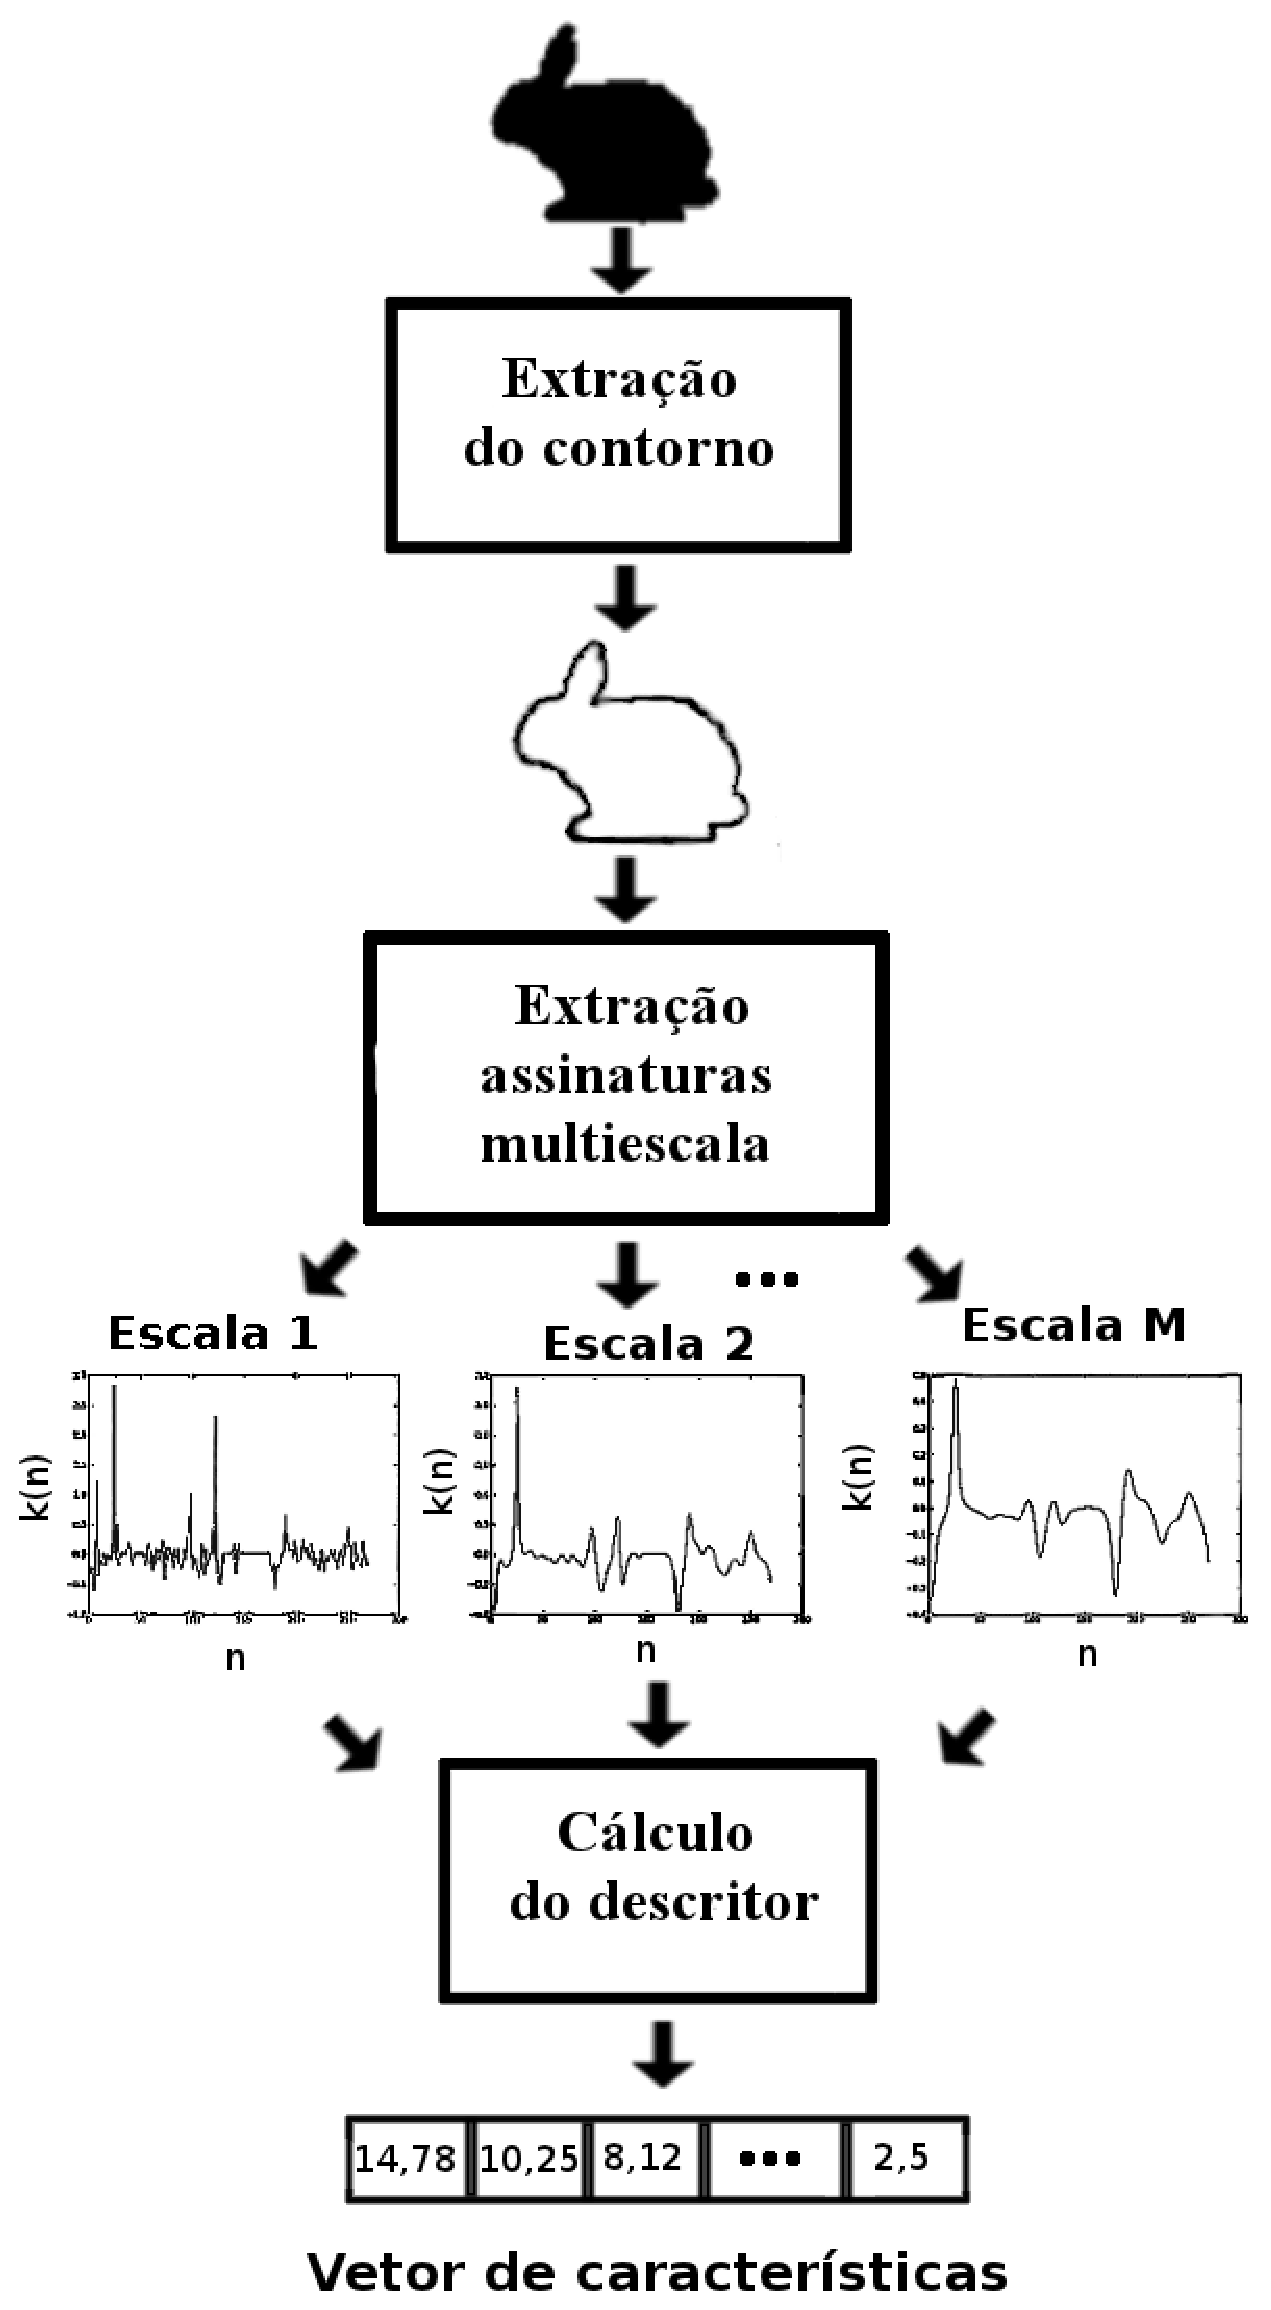
\includegraphics[width=0.45\textwidth]{feature_extraction.eps}
 % \legend{Fonte: próprio autor}
\end{figure}

A Figura \ref{fig:ms} ilustra o processo para obtenção de uma representação multiescala de um sinal unidimensional discreto $k[n]$ que represente o contorno de uma forma, tal como as assinaturas apresentadas na Subseção \ref{sec:Assinatura}. Emprega-se nesse processo uma função de transformação $F[n,\sigma]$, geralmente com características de filtragem passa-baixas e com frequência de corte $\sigma$. Na função de transformação, a referida frequência de corte corresponde ao fator de escala na qual o sinal $k[n]$ será analisado. 

Para um vetor de escalas $\sigma = (\sigma_1\:\sigma_2\:\ldots\:\sigma_M) $, a representação multiescala consiste em um vetor de sinais $k[n,\sigma] = (k[n,\sigma_1]\:k[n,\sigma_2]\:\ldots\:k[n,\sigma_N])$, sendo cada termo $k[n,\sigma_i]$ obtido através de
\begin{equation}\label{eq:ms1}
k[n,\sigma_i] = F[n,\sigma_i]*k[n]\text{,}
\end{equation}

\noindent
 aonde o operador $*$ denota a convolução entre o sinal $k[n]$ e a transformação $F[n,\sigma_i]$.  Assim, cada elemento de $k[n,\sigma]$ corresponde ao sinal $k[n]$ analisado na escala $\sigma_i$.

No caso de curvas planas, a análise multiescala permite descrevê-las em vários níveis de detalhes e de abstração a partir de suas assinaturas, tornando a representação mais discriminativa que os métodos que empregam medidas quantitativas globais, como área, perímetro e compacidade, devido a sua robustez e estabilidade \cite{4756134}.    

\subsubsection*{Curvatura Multiescala\label{subsec:curvMS}}

Inspirados na técnica de \citeonline{Witkin:1983} e \citeonline{Koenderink:1984}, \citeonline{149591} propuseram um método para análise multiescala do contorno através da assinatura da curvatura. O referido método emprega como função de transformação um filtro passa-baixas gaussiano, $g_{\sigma}(l) = \frac{1}{\sigma\sqrt{2\pi}}e^{\frac{l^2}{2\sigma^2}}$, que suaviza o contorno antes do cálculo de sua curvatura. Nesse caso, o ajuste do desvio padrão da função gaussiana ($\sigma^2$) atua como fator de escala, regulando a largura de banda do filtro e o nível de suavização do contorno.

%Desta forma, o sinal da curvatura é obtido em múltiplas escalas uma vez que a suavização do contorno possibilita o cálculo das derivadas. 


No caso contínuo temos as coordenadas do contorno suavizado realizando a convolução entre as coordenadas do contorno parametrizado $C(l) = (x(l)\text{,}y(l))$ e o filtro gaussiano:  

\begin{equation}
x_{\sigma}(l) = x(l) * g_{\sigma}(l) = \int^{\infty}_{-\infty}{x(v)g_{\sigma}(l-v)}dv \text{ e}
\end{equation}
\begin{equation}
y_{\sigma}(l) = y(l) * g_{\sigma}(l)=\int^{\infty}_{-\infty}{y(v)g_{\sigma}(l-v)}dv
\end{equation}\text{.}

Para o cálculo das derivadas $x^{'}_{\sigma}(l)\text{, }y^{'}_{\sigma}(l)\text{, }x^{''}_{\sigma}(l) \text{ e }y^{''}_{\sigma}(l)$, necessárias para o cálculo da curvatura do contorno suavizado, temos, pelas propriedades da convolução, $x^{'}_{\sigma}(l) = x(l) * g^{'}_{\sigma}(l)\text{, }y^{'}_{\sigma}(l) = y(l) * g^{'}_{\sigma}(l)\text{, }x^{''}_{\sigma}(l) = x(l) * g^{''}_{\sigma}(l)\text{ e }
y^{''}_{\sigma}(l) = y(l) * g^{''}_{\sigma}(l)$.

O cálculo da curvatura do contorno suavizado $K_{\sigma}(l)$ se dá através da equação \ref{eq:curvatura}, substituindo-se $x^{'}(l)\text{, }\:y^{'}(l)\text{, }\:x^{''}(l)\:\text{ e }\:y^{''}(l)$ por $x^{'}_{\sigma}(l)\text{, }\:y^{'}_{\sigma}(l)\text{, }\:x^{''}_{\sigma}(l)\:\text{ e }\:y^{''}_{\sigma}(l)$, respectivamente, ou seja,

\begin{equation} \label{eq:curvatura_ms}
K_{\sigma}(l) = \frac{x_{\sigma}^{'}(l)y_{\sigma}^{''}(l)-x_{\sigma}^{''}(l)y_{\sigma}^{'}(l)}{((x_{\sigma}^{''}(l))^{2}+(y_{\sigma}^{''}(l))^{2})^{\frac{3}{2}}}\text{.}
\end{equation}

Uma outra abordagem utilizada para se calcular a curvatura multiescala, que foi proposta por \citeonline{Cesar:1996} e adotada nesta tese, opera com a representação do contorno no domínio da frequência. A partir da transformada de Fourier das coordenadas do contorno suavizado $X_{\sigma}(f) = F\big\{x_{\sigma}(l)\big\}$ e $Y_{\sigma}(f) = F\big\{y_{\sigma}(l)\big\}$. Os referidos autores calculam derivadas utilizando a propriedade da derivada da transformada de Fourier, ou seja:

\begin{equation}
x_{\sigma}^{'}(l) = F^{-1}\big\{2 \pi j f  X_{\sigma}(f)\big\}
\end{equation}

\begin{equation}
y_{\sigma}^{'}(l) = F^{-1}\big\{2 \pi j f  Y_{\sigma}(f)\big\}
\end{equation}

\begin{equation}
x_{\sigma}^{''}(l) = F^{-1}\big\{- (2 \pi f)^2 X_{\sigma}(f)\big\}
\end{equation}

\begin{equation}
y_{\sigma}^{''}(l) = F^{-1}\big\{- (2 \pi f)^2 Y_{\sigma}(f)\big\}
\end{equation}, aonde $F^{-1}\big\{X(f)\big\}$ denota a transformada de Fourier inversa do sinal $X(f)$.

\begin{comment}
\begin{equation}
X(f) = F\big\{x(l)\big\} = \int\limits^\infty_\infty x(l)e^{-2 \pi j f l}dl
\end{equation}

\begin{equation}
x(l) = F^{-1}\big\{X(f)\big\} \int\limits^\infty_\infty X(f)e^{2 \pi j f l}df
\end{equation}
\end{comment}

Na suavização do contorno no domínio da frequência, ao invés da convolução, realiza-se o produto dos sinais $X(f)$ e $Y(f)$ com a transformada de Fourier da expressão do filtro gaussiano:

\begin{equation}
X_\sigma(f) = X(f).G_\sigma(f)
\end{equation}

\begin{equation}
Y_\sigma(f) = Y(f).G_\sigma(f)
\end{equation}, sendo

\begin{equation}
G_\sigma(f) = F\big\{ g_{\sigma}(l)\big\} = e^{-2 \pi^2 f^2 \sigma^2}\text{.}
\end{equation}

\begin{figure}[h!]
  \caption{\label{fig:curv_ms} Curvatura multiescala do contorno da folha da Figura \ref{fig:folha_contorno1}.}
  \centering
  \includegraphics[width=0.75\textwidth]{curvograma_v2.png}
 \end{figure}

A Figura \ref{fig:curv_ms} ilustra a evolução do sinal de curvatura do contorno da folha da Figura \ref{fig:folha_contorno1} para diferentes níveis de suavização. Os picos da curvatura que se preservam nas escalas de baixa resolução correspondem às informações mais salientes do contorno, que o caracterizam globalmente. As informações de detalhes, que tendem a desaparecer nas escalas de baixa resolução e se preservam nas escalas de alta resolução, representam as características mais especificas do contorno.

{\color{blue}
\citeonline{Costa:1997} propuseram um método para o ajuste das escalas através das expressões

\begin{equation}
oct_l = (\sqrt{2})^l;\text{ }l = 1,\ldots,S
\end{equation} 
\noindent e
\begin{equation}
\sigma_l = \big(\frac{\sigma_{max} - \sigma{min}}{oct_{max}-\sqrt{2}}\big)(oct_l - \sqrt{2})+\sigma_{min}\text{,}
\end{equation}

\noindent aonde $S$ é o número de escalas, $l$ a l-ésima escala calculada $\sigma_{min} = \sigma_1$ a menor escala e $\sigma_{max} = \sigma_S$ a maior escala.
}
 
\subsubsection*{Dimensão Fractal multiescala (DFM)}

O conceito de fractal, introduzido por \citeonline{Mandelbrot:2000}, está intimamente relacionado com a auto-similaridade ou escala de uma forma, o que por sua vez estabelece a noção de dimensão fractal.

Tanto a dimensão fractal como a dimensão fractal multiescala permitem estimar a complexidade de uma forma \cite{Backes:2012}. Complexidade é uma propriedade importante das formas que informa quanto espaço uma determinada forma ocupa \cite{Costa:2009}. A dimensão fractal multiescala estima a complexidade da forma através de uma curva que representa as mudanças na complexidade à medida que a escala de visualização da forma varia \cite{Florindo:2012}.

Nesta tese o método empregado para estimar a dimensão fractal e a dimensão fractal multiescala é o método de Minkowski-Bouligand \cite{Costa:2009}. Este método dilata a forma sob análise utilizando como elemento estruturante um disco de raio $r > 0$, sucessivamente. A inclinação da interpolação linear da curva $\log{A(r)}$ versus $\log{r}$ determina a estimativa da dimensão fractal $D_f$, que é dada por:

\begin{equation}
D_f = 2 - \lim_{r \to 0}  \frac{\log{A(r)}}{\log{r}}.
\label{eq:df}
\end{equation}

A derivada da curva log-log, representada através de $N$ valores discretos de raios $r_i>0$, determina a dimensão fractal multiescala:

\begin{equation}
DFM = \big(D_f(t_1)\text{, }D_f(t_2)\text{, }\ldots\text{ , }D_f(t_N)\big), 
\label{eq:dfm}
\end{equation}

\noindent aonde  $D_f(t) = 2 - \frac{du(t)}{dt}$, $t = \log{r}$ e $u(t) = \log{A(t)}$.


\section{Técnicas de visualização de dados}

Um problema dos algoritmos empregados na extração de características, que foram abordados nesse capítulo é a elevada dimensionalidade da representação vetorial obtida. Além de dificultar compreender a organização dos dados, essa elevada dimensionalidade acarreta em maior complexidade do sistema computacional que deve lidar com essa informação. 

Através de técnicas de redução de dimensionalidade é possível gerar visualizações gráficas dos dados, o que permite compreender melhor sua estrutura. Ademais, tais técnicas removem informações redundantes e irrelevantes, reduzindo assim a complexidade da representação obtida.

Apresentamos neste capítulo duas técnicas de visualização de dados que foram empregadas neste trabalho na avaliação da capacidade discriminativa dos descritores do contorno de formas: a análise das componentes principais (\emph{PCA}) e o mapa auto-organizável de Kohonen (SOM).

%Essas técnicas foram aplicadas aos descritores energia de dobramento multiescala, dimensão fractal multiescala, entropia diferencial multiescala e entropia discreta multiescala. Limitamos esse estudo a tais descritores porque os mesmos representam as formas através de vetores de características de mesma dimensão, que é um requisito para a aplicação das técnicas de visualização estudadas.

%Essas técnicas tem em comum a propriedade de projetar os dados de dimensionalidade elevada em um espaço bidimensional. 

\subsection{Análise das componentes principais (PCA)}

\begin{figure}[h!]
  \caption{\label{fig:nuvem_pca} Projeções das três primeiras componentes principais dos vetores de características obtidos  a partir do descritor \emph{NMBE} e os vetores transformados através de \emph{PCA}.}
  \centering
  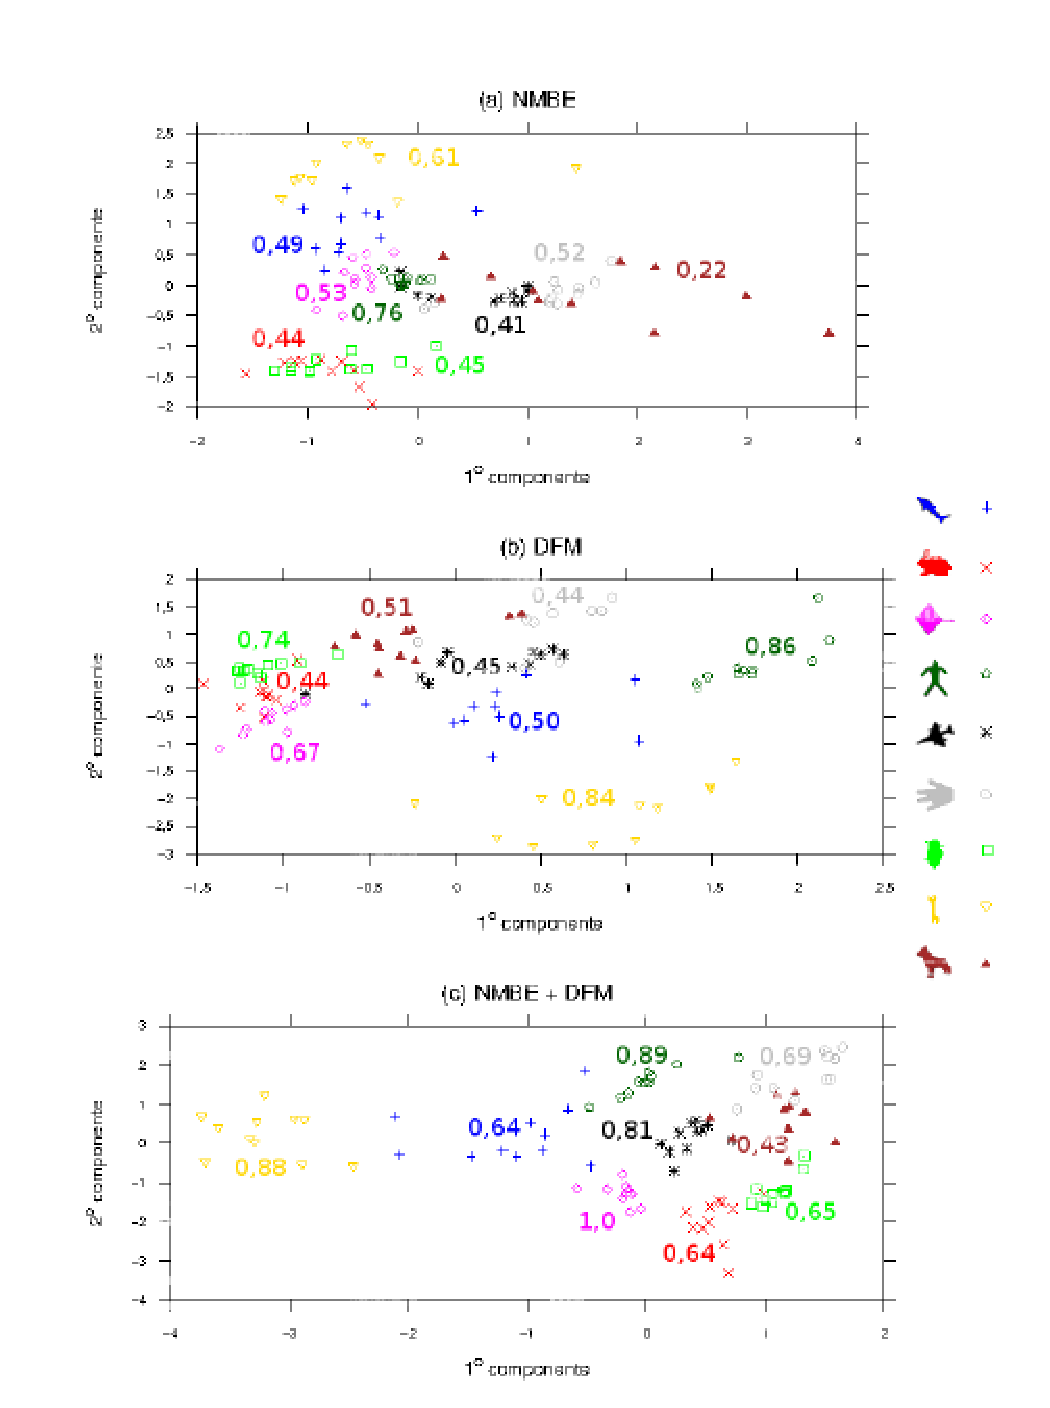
\includegraphics[width=0.75\textwidth]{nuvem_pca.eps}
\end{figure}

O propósito da análise das componentes principais é obter um conjunto de variáveis não correlacionadas, em ordem decrescente de importância, a partir da combinação linear das variáveis originais. Sob o aspecto geométrico, esse processo de combinar linearmente as variáveis pode ser entendido como realizar a rotação dos eixos do sistema de coordenadas original, a fim de se encontrar um novo sistema de coordenadas ortogonal em que as variáveis transformadas apresentem máxima variância. 

Desde que a maior parte da variância esteja concentrada nas primeiras componentes das variáveis transformadas, consegue-se obter através dessa técnica uma representação com um número reduzido de variáveis.

A técnica \emph{PCA} é não supervisionada, pois não leva em consideração informação a priori dos agrupamentos, ou rótulos, dos dados.  Sendo a transformação \emph{PCA} linear, temos que

\begin{equation}\label{eq:PCA1}
\mathbf{y}=\mathbf{A}^T\mathbf{x}
\end{equation}

\noindent aonde $ \mathbf{A} = \begin{pmatrix}
  a_{1,1} & a_{2,1} & \cdots & a_{p,1} \\
  a_{1,2} & a_{2,2} & \cdots & a_{p,2} \\
  \vdots  & \vdots  & \ddots & \vdots  \\
  a_{1,p} & a_{2,p} & \cdots & a_{p,p}
 \end{pmatrix} = 
 \begin{pmatrix}
 \mathbf{a_{1}}&
 \mathbf{a_{2}}&
 \cdots&
 \mathbf{a_{p}}
 \end{pmatrix}$ é a matriz de transformação, $\mathbf{x} = \begin{pmatrix} x_1&x_2&\ldots&x_p\end{pmatrix}^T$ e $\mathbf{y} = \begin{pmatrix}y_1&y_2&\ldots&y_p\end{pmatrix}^T$ vetores de variáveis aleatórias e $\mathbf{a_1}\text{ a }\mathbf{a_p}$ vetores dos coeficientes da base de transformação.
 
Logo, cada variável de saída $y_i$ é obtida através da combinação linear das variáveis de entrada pela seguinte equação:
 
 \begin{equation}\label{eq:PCA2}
 y_i = \sum\limits_{j = 1}^p a_{i,j}x_j = \mathbf{a_i}^T\mathbf{x}
 \end{equation}

Pode-se demonstrar que, para se obter em $\mathbf{y}$ variáveis que não são correlacionadas,  deve-se atribuir aos vetores de coeficientes $\mathbf{a_1} \ldots \mathbf{a_p}$ os auto-vetores da matriz de covariância de $\mathbf{x}$, sendo esta última dada por: 

\begin{equation}\label{eq:PCA3}
\mathbf{\Sigma_x} = E{[\mathbf{xx}^T]}-E{[\mathbf{x}]}E{[\mathbf{x}^T]}
\end{equation}

\noindent aonde $E[.]$ denota o operador esperança. 
Já que $\mathbf{\Sigma_x}$ é de dimensão $p \times p$, temos associada a esta $p$ auto-vetores ($\mathbf{a_1}\text{, }\mathbf{a_2}\text{, }\ldots\text{, }\mathbf{a_p}$) com $p$ auto-valores ($\lambda_1 > \lambda_2 \ldots > \lambda_p$) correspondentes, sendo cada auto-valor $\lambda_i$ a variância de cada variável de saída $y_i$ obtida através da Equação \ref{eq:PCA2}. 

Selecionando dentre as componentes somente aquelas de maior variância, que implica em construir a matriz de transformação apenas com os auto-vetores mais significativos, é possível obter uma representação dos dados em um espaço de dimensão reduzida e de mais fácil entendimento do ponto de vista geométrico.

Na Figura \ref{fig:nuvem_pca} temos representadas as projeções das duas componentes principais de maior variância para cada um dos descritores avaliados. Os valores numéricos correspondem a taxa de acerto média nos experimentos de recuperação de formas pelo conteúdo alcanças para cada classe de formas representada.

\subsection{Escalonamento multidimensional (\emph{MDS})}

O escalonamento multidimensional \cite{cox:2000} consiste em um método para representação de dados de um espaço inicial, multi dimensional, para um espaço de dimensão reduzida, preservando as relações de distâncias existentes no espaço inicial. Esse algoritmo modela a similaridade ou disimilaridade dos dados como distâncias no espaço geométrico.

Há dois tipos de algoritmos \emph{MDS}: o métrico e o não métrico. No primeiro, a matriz de similaridade de entrada é construída a partir de uma métrica de distância que respeita a desigualdade triangular. Assim, as distâncias entre dois pontos no espaço de dimensão reduzida são ajustadas para serem  mais próximas possível àquelas encontradas no espaço de dimensão inicial. Em sua versão não métrica, o algoritmo tenta preservar a ordem das distâncias, procurando uma relação monotônica não paramétrica entre as proximidades das distâncias do espaço de dimensão reduzida e as similaridades no espaço de dimensão inicial.

O coeficiente $R^2$ mede o ajuste da representação dos dados em um espaço de menor dimensão. Este coeficiente indica, em porcentagem, o ajuste do modelo aos dados observados. Assim, quando mais próximo de 1 o valor de $R^2$, melhor o ajuste do modelo aos dados observados.  Sejam $d$ e $\hat{d}$ as matrizes de distância simétricas entre dois vetores nos espaços de menor e maior dimensão, respectivamente. O coeficiente $R^2$ é dado por 
\begin{equation}
R^2= 1-\frac{\sum_{i=1}^n \sum_{j = i}^{n}(\hat{d}_{i,j} - d_{i,j})^2}{\sum_{i=1}^n\sum_{j=i}^n (d_{i,j}-\bar{d})^2}
\text{,}\:\: R^2 \in [0,1]
\end{equation}

\noindent em que  $n$ é o número de amostras, $d_{i,j}$ é a distância entre as amostras $i$ e $j$ no espaço de mais alta dimensão, $\hat{d}_{i,j}$ é a distância entre as amostras $i$ e $j$ no espaço de menor dimensão e $\bar{d}$  é a distância média no espaço de mais alta dimensão.



\subsection{Mapa auto-organizável de Kohonen}

O mapa auto-organizável de Kohonen, ou rede \emph{SOM} \cite{Kohonen:2001}, consiste em um tipo de rede neural de aprendizagem não supervisionada. Desenvolvida por \citeonline{Kohonen:1982}, a rede \emph{SOM} projeta os vetores apresentados em sua entrada de um espaço N-dimensional para um espaço bidimensional, preservando a estrutura topográfica do espaço vetorial de origem. Em outras palavras, se dois vetores encontram-se próximos no espaço de entrada, estes preservarão essa relação de proximidade no espaço de projeção. 

\begin{comment}
Em seu processo de treinamento, a rede \emph{SOM} agrupa os vetores de entrada através de um processo de aprendizado competitivo mantendo a estrutura topológica do espaço vetorial de entrada.
\end{comment}

Sendo uma ferramenta para análise exploratória de dados, esse tipo de rede neural tem sido empregada para visualização de imagens \cite{Strong2011774}, identificação de agrupamentos \cite{Kuroiwa200031}, classificação de texturas \cite{595364}, bem como outras aplicações.

\citeonline{Ultsch:1990} demonstraram que, embora a rede \emph{SOM} organize os vetores em agrupamentos, esta não representa as distâncias entre os mesmos de maneira fidedigna. Isso torna a análise direta do mapa de projeções não adequada para a análise dos agrupamentos estabelecidos. 

Para contornar esse problema, os referidos autores desenvolveram um método bidimensional de representação conhecido como matriz unificada de distâncias ou matriz-U. Obtida a partir do mapa \emph{SOM} essa matriz mostra, preservando a topologia, a relação de distância entre as estruturas mapeadas \cite{Ultsch:1990}. 

Para ilustrarmos como se interpreta a informação contida na matriz-U apresentamos como exemplo a imagem da Figura \ref{fig:u-matrix}. Nesta imagem a matriz-U é representada por um conjunto de células em níveis de cinza. As estruturas claras rotuladas representam os neurônios da rede SOM, enquanto as demais células representam o grau de separação existente entre as estruturas. Células mais escuras representam maior grau de separação entre as estruturas mapeadas pela matriz. Já células mais claras, tais como as que tendem ao branco, representam maior grau de proximidade entre as estruturas mapeadas. 

\begin{figure}[]
  \caption{\label{fig:u-matrix} Representação da Matriz-U como imagem em níveis de cinza. As células brancas rotuladas correspondem aos neurônios da rede SOM. Células escuras indicam maior separação entre neurônios e células claras indicam maior proximidade entre neurônios.}
  \centering
  \includegraphics[width=0.4\textwidth]{u-matrix_gray.png}
\end{figure}

Interpretando esta figura observamos que as estruturas A5, A4 e A8 estão bem próximas umas das outras. Já a estrutura A9 encontra-se afastada das referidas estruturas. Dada a grande separação existente entre as quatro estruturas analisadas e as demais estruturas da matriz (E8, E6, E10, E9, E3 e B9), podemos inferir que as quatro estruturas (A5, A4, A8 e A9) formam um agrupamento. Já as estruturas E8, E6, E10 e E9 formam um outro agrupamento, embora não estejam tão próximas umas das outras como no caso anterior. Quanto às estruturas B9 e E3, estas estão isoladas, ou seja, muito distante das demais estruturas da matriz.

\begin{comment}

The concept of fractal, introduced by Mandelbrot \citep{Mandelbrot:2000}, is closely related to self-similarity or scaling of a shape. Moreover, it encompasses the notion of fractional dimension.  Actually, fractal dimension and \emph{MFD} are well-known methods to estimate shape complexity \citep{Backes:2012}. Shape complexity is an important concept in shape analysis that informs how much space a shape occupies \cite{Costa:2009}. \emph{MFD} estimates shape complexity through a curve that represents changes in the complexity as the shape visualization scale varies \cite{Florindo:2012}. 

%and for feature extraction of biological forms %\citep{Rossatto:2011}.  In fact, it quantifies the %self-similarity of a shape.

% quantifica a aspereza ou rugosidade de uma forma \citep{Schroreder:1996}.\\

%Uma das caracter\'isticas das formas fractais \'e a sua auto-similaridade \citep{Schroreder:1996}. Isso significa que uma forma, tanto em escalas menores como maiores, \'e constitu\'ida por um mesmo conjunto de primitivas $D_f$.\\

%Qualquer forma auto-similar pode ser dividida em $N$ partes auto-similares, ou seja, c\'opias menores que sejam escalonadas por um fator $b$, atrav\'es da equa\c c\~ao:\\

%\begin{equation}
%D_{f} = \frac{\log{N}}{\log{\frac{1}{b}}}.
%\label{eq:dfc}
%\end{equation}

%Esse descritor pode ser construído a partir do método de Bouligand-Minkowski de estimação da dimensão fractal ($D_f$) \citep{Costa:2009}. Utilizado em \citep{Florindo:2012} e \citep{Backes:2012}, o referido método aplica dilatações exatas à  forma analisada tendo como elemento estruturante uma região circular de raio $r > 0$. O coeficiente angular da interpolação linear da curva $\log{A(r)}$ versus $\log{r}$ é utilizado como uma estimativa da $D_f$:

In this paper, the Minkowski-Bouligand method estimates the fractal dimension ($D_f$) \citep{Costa:2009} and hence the \emph{MFD} descriptor. This estimation method dilates the shape under analysis  using a disk structuring element of radius $ r>0 $, successively. The slope of the linear interpolation of the curve $\log{A(r)}$ versus $\log{r}$ provides the $D_f$ estimation, given by: 

\begin{equation}
D_f = 2 - \lim_{r \to 0}  \frac{\log{A(r)}}{\log{r}}.
\label{eq:df}
\end{equation}
%O cálculo da MFD decorre do calculo da derivada da curva log-log, obtida a partir da equação \ref{eq:df}, para diferentes valores de raios $r$:
Then, the derivative of th log-log curve for $N$ discrete values of radii $r_i>0$ gives 

\begin{equation}
MFD = \big(D_f(t_1)\text{, }D_f(t_2)\text{, }\ldots\text{ , }D_f(t_N)\big), 
\label{eq:dfm}
\end{equation}

\noindent where  $D_f(t) = 2 - \frac{du(t)}{dt}$, $t = \log{r}$ and $u(t) = \log{A(t)}$.

\end{comment}

\section{Métodos de otimização}

Problemas de otimização, que consistem em encontrar mínimo e máximo de uma função objetivo de múltiplas variáveis, ocorrem com frequência em diversas áreas do conhecimento, como engenharia, economia e ciências. Métodos clássicos,{\color{red} PRECISA CITAR UMA FONTE AQUI como o de Newton-Rapson }e suas variantes, funcionam muito bem no caso em que a função objetivo é diferenciável e com um único ótimo global no entanto, tais condições não são encontradas em diversos problemas. 

Os métodos de otimização evolutivos foram desenvolvidos para lidar com o problema de otimização de funções de múltiplas  variáveis, não diferenciáveis e com ótimos locais. Inspirados nos processos biológicos evolutivos, esses métodos utilizam de metaheurísticas e uma população de soluções candidatas para realizar buscas no espaço de pesquisa pela solução ótima. Esta seção apresenta três algoritmos metaheurísticos de otimização que foram utilizados nesta tese no ajuste de parâmetros dos descritores multiescala: evolução diferencial  \cite{Storn:1007}, enxame de partículas  \cite{Yuhui:1998} e recozimento simulado \cite{Andries:2007}.
%This paper investigates three optimization algorithms to search for the best solution that minimizes the objective function MAD: the simulated annealing (SA) \cite{Andries:2007}, differential evolution (DE) \cite{Storn:1007} and particle swarm (PSO) \cite{Yuhui:1998}. 
\subsection{Recozimento simulado (\emph{SA})}

O  recozimento simulado é um método clássico de otimização metaheurístico que simula o processo termodinâmico de aquecimento e resfriamento de um metal. O mecanismo desse método para exploração do espaço de busca consiste numa variável de temperatura que determina a probabilidade de aceitação de uma solução pior àquela encontrada até o momento, sendo que quanto maior for a termperatura, maior será essa probabilidade. Soluções melhores que a solução atual são sempre aceitas pelo algoritmo, enquanto que a probabilidade de aceitar soluções piores descresce exponencialmente à medida que o algoritmo interage.  

Na exploração do espaço de busca, esse algoritmo também requer um mecanismo de perturbação da solução atual, que consiste em adicionar ou subtrair, com uma dada probabilidade $P_r$, um fator de perturbação aleatório a cada coordenada da solução atual. Na implementação utilizada neste trabalho, o fator de perturbação corresponde a uma variável aleatória com distribuição normal com média zero e variância $\kappa = 0.2$.

\begin{algorithm}[ht]
\caption{Simulated Annealing}
\label{alg:sa}
\begin{algorithmic}
\Require $N\text{,}\:M\text{,}\:T_0\text{,}\:P\text{,}\:L> 0$, $:\alpha\text{,}\:\kappa\text{,}\:P_r \in [0,1]$, $\:COST$.
\Ensure The best found solution that minimizes $COST$.

\Function{DISTURB}{$\boldsymbol{v}$}
\State $f \gets$ \Call{$COST$}{$\boldsymbol{v}$}
\For{$i = 0,\:1,\:\cdots,\:M-1$} 
\If {$P_r > U(0,1)$}
\State $aux \gets v[i]$
\State $v[i] \gets v[i]+ \kappa.(1+f).\mathcal{N}(0,1).v[i]$
\If {$v[i] \notin [0.125,125.5]$}
\State $v[i] \gets aux$
\EndIf
\EndIf
\EndFor
\State \Return $\boldsymbol{v}$
\EndFunction

\State $i \gets 1$, $n \gets 0$,$T \gets T_0$
\For{$j = 0,\:1,\:\cdots,\:M-1$} 
\State $s[j] \gets U(0.125,125.5)$
\EndFor
\State $fit \gets$ \Call{$COST$}{$\boldsymbol{s}$} 
\Repeat
\State $\boldsymbol{s_d} \gets$ \Call{$Disturb$}{$\boldsymbol{s}$}
\State $\delta \gets$ \Call{$COST$}{$\boldsymbol{s_d}$}$- fit$ 
\If {$\delta < 0$ or $\exp{(\frac{\delta}{T})} > U(0,1)$}
\State $\boldsymbol{s} \gets \boldsymbol{s_d}$,$fit \gets $ \Call{$COST$}{$\boldsymbol{s_d}$}
$n \gets n + 1$
\EndIf
\State $i \gets i + 1$
\Until{$i > P$ or $n > L$}
\State $T \gets \alpha.T$
\end{algorithmic}
\end{algorithm}

\subsection{Evolução diferencial \emph{DE}}

O algoritmo de otimização evolução diferencial \cite{Storn:1996} emprega mecanismos de cruzamento e mutação de espécies para evoluir uma população de $N$ indivíduos ou vetores de soluções candidatas. A cada interação, o mecanismo de cruzamento e mutação  se dá para cada indivíduo da população. O cruzamento consiste em produzir uma novo indivíduo ($d$) a partir de três indivíduos distintos sorteados da população $\boldsymbol{\sigma_1}$, $\boldsymbol{\sigma_2}$ e $\boldsymbol{\sigma_3}$ que sejam diferentes do individuo atualmente em evolução $(\boldsymbol{\sigma_k}$). Para a variante do algoritmo \emph{DE/rand/1} \cite{Storn:1996}, a regra de cruzamento é  

\noindent
\begin{equation}
\label{eq:de}
\boldsymbol{d} = \boldsymbol{\sigma_1} + \beta.(\boldsymbol{\sigma_2} - \boldsymbol{\sigma_3}),
\end{equation}

\noindent sendo o parâmetro $\beta$ um fator de amplificação da diferença entre os vetores $\boldsymbol{\sigma_2}$ e $\boldsymbol{\sigma_3}$.

O mecanismo de mutação do \emph{DE} utiliza o indivíduo $\boldsymbol{d}$, produzido pela Equação \ref{eq:de}, para perturbar o vetor de solução candidata atualmente em evolução $\boldsymbol{\sigma_k}$. Assim, com probabilidade de mutação $P_r$, substitui-se cada coordenada de $\boldsymbol{\sigma_k}$ pela coordenada de $\boldsymbol{d}$ correspondente. A implementação do \emph{DE} está detalhada no Algoritmo \ref{alg:de}.

\begin{algorithm}[ht]
\caption{Differential evolution optimization}
\label{alg:de}
\begin{algorithmic}
\Require $N\text{,}\:M > 0$, $\:\beta\text{,}\:P_r \in (0,1]$, $\:COST$
\Ensure The best found solution that minimizes $COST$
\For{$i = 0,\:1,\:\cdots,\:N-1$}
\For{$j = 0,\:1,\:\cdots,\:M-1$}
\State $\boldsymbol{pop}[i][j] \gets U(0.125,125.0)$
\EndFor
\EndFor

\For{$j = 0,\:1,\:\cdots,\:1250$}
\For{$i = 0,\:1,\:\cdots,\:N-1$}
\State Select in $\boldsymbol{pop}$ three random distinct candidate solutions ($\boldsymbol{\sigma_a}$, $\boldsymbol{\sigma_b}$ and $\boldsymbol{\sigma_c}$) that differ from $\boldsymbol{pop}[i]$
\State $\boldsymbol{d} \gets \boldsymbol{\sigma_a} + \beta.(\boldsymbol{\sigma_b} - \boldsymbol{\sigma_c})$
\For{$k = 0,\:1,\:\cdots,\:M-1$}
\If{$\boldsymbol{d}[k] \notin [0.125,125.0]$}
\State $\boldsymbol{d}[k] \gets U(0.125,125.0)$
\EndIf
\EndFor
\State $\boldsymbol{c} \gets \boldsymbol{pop}[i]$
\State $k \gets U(0,M-1)$
\State $c[k] \gets d[k]$
\For{$k = 0,\:1,\:\cdots,\:M-1$}
\If {$U(0,1) \leq P_r$}
  \State $c[k] \gets d[k]$
\EndIf
\EndFor

\If {\Call{$COST$}{$\boldsymbol{c}$} $<$ \Call{$COST$}{$\boldsymbol{pop}[i]$}}
 \State $\boldsymbol{pop}[i] \gets \boldsymbol{c}$
\EndIf
\EndFor
\EndFor
\end{algorithmic}
\end{algorithm}

\subsection{Enxame de partículas (\emph{PSO})}
 O enxame de partículas é um algoritmo de otimização bio-inspirado que evolui uma população de $N$ partículas que se movimentam no espaço de busca a uma dada velocidade. A cada interação o algoritmo \emph{PSO}: a) registra as melhores posições alcançadas por cada partícula (\emph{bpp}) e a melhor posição globalmente encontrada por todas as partículas do enxame (\emph{bgp}); b) corrige a velocidade das partículas considerando dois fatores de atração $c_1$ e $c_2$. O primeiro fator controla a tendência da partícula procurar a solução ótima nas redondezas de \emph{bpp} e o segundo a tendência da partícula se movimentar em direção a \emph{bgp}; c) Atualiza a posição das partículas a partir das suas velocidades.
 
 Para melhorar a convergência a um mínimo global, as partículas são desaceleradas exponencialmente  a cada interação por um fator de inércia $\omega$ \cite{Yuhui:1998}. O ajuste dos parâmetros do algoritmo $PSO$ é um aspecto importante a ser considerado. Um estudo das características de convergência do algoritmo, bem como recomendações de ajuste dos parâmetros com base nessas características  é encontrado em \cite{Jiang20078}. O Algoritmo \label{alg:pso} detalha a implementação do \emph{PSO} 
  
  
\begin{algorithm}[ht]
\caption{Particle Swarm Optimization \label{alg:pso}}

\begin{algorithmic}
\Require $N\text{,}\:M > 0$,  $\:\omega \in (0,1]$, $\:c_1\text{,}\:c_2 \in R^+ $, $\:COST$
\Ensure The best found solution that minimizes $COST$
\For{$i = 0,\:1,\:\cdots,\:N-1$}
\For{$j = 0,\:1,\:\cdots,\:M-1$}
\State $pop[i][j] \gets U(0.125,125.5)$ 
\State $v[i][j] \gets U(0.125,125.5)$
\EndFor
\State $fit[i] \gets$ \Call{$COST$}{$\boldsymbol{pop}[i]$}
\State $\boldsymbol{bpp}[i] \gets \boldsymbol{pop}[i]$ 
\EndFor
\State $\boldsymbol{bgp} \gets \boldsymbol{bpp}[argmin(\boldsymbol{fit})]$
\For{$i = 0,\:1,\:\cdots,\:1250$}
\For{$j = 0,\:1,\:\cdots,\:N-1$}
\State $\boldsymbol{v}[j] \gets \omega.\boldsymbol{v}[j]$
\State $\boldsymbol{v}[j] \gets \boldsymbol{v}[j] + c1.U(0,1).(\boldsymbol{pop}[j] - \boldsymbol{bpp}[j])$
\State $\boldsymbol{v}[j] \gets \boldsymbol{v}[j] + c2.U(0,1).(\boldsymbol{pop}[j] - \boldsymbol{bgp})$
\State $\boldsymbol{pop}[j] \gets \boldsymbol{pop}[j] + \boldsymbol{v}[j]$
\For{$k = 0,\:1,\:\cdots,\:M-1$}
\If{$pop[j][k] \notin [0.125,125.0]$}
\State $pop[j][k] \gets U(0.125,125.0)$
\EndIf
\EndFor
\State $fit[j] \gets$ \Call{$COST$}{$\boldsymbol{pop}[j]$}
\If {$fit[j] <$ \Call{$COST$}{$\boldsymbol{bpp}[j]$}} 
\State $\boldsymbol{bpp}[j] \gets \boldsymbol{pop}[j]$
\EndIf
\If {\Call{$COST$}{$\boldsymbol{bpp}[j]$} $<$ \Call{$COST$}{$\boldsymbol{bgp}$}}
\State $\boldsymbol{bgp} \gets \boldsymbol{bpp}[j]$
\EndIf
\EndFor
\EndFor
\end{algorithmic}
\end{algorithm}
